% Chapter Template

\chapter{MODI} % Main chapter title

\label{Chapter3} % Change X to a consecutive number; for referencing this chapter elsewhere, use \ref{ChapterX}

\lhead{Capítulo 3. \emph{MODI}} % Change X to a consecutive number; this is for the header on each page - perhaps a shortened title

%----------------------------------------------------------------------------------------
%	SECTION 1
%----------------------------------------------------------------------------------------

\section{Setup}

Se desea hacer realizar una investigación sobre el comportamiento colectivo de un grupo de robots, en el mundo real sin hacer uso de simuladores. Por esto  es necesario contar con un lugar físico donde poder activar los robot. Además para simplificar cada uno de los robots, estos no tienen sensores internos por lo que hay una cámara montada sobre el plano de movimiento de los robots, para hacer Seguimiento Visual.
\begin{figure}[htbp]
	\centering
		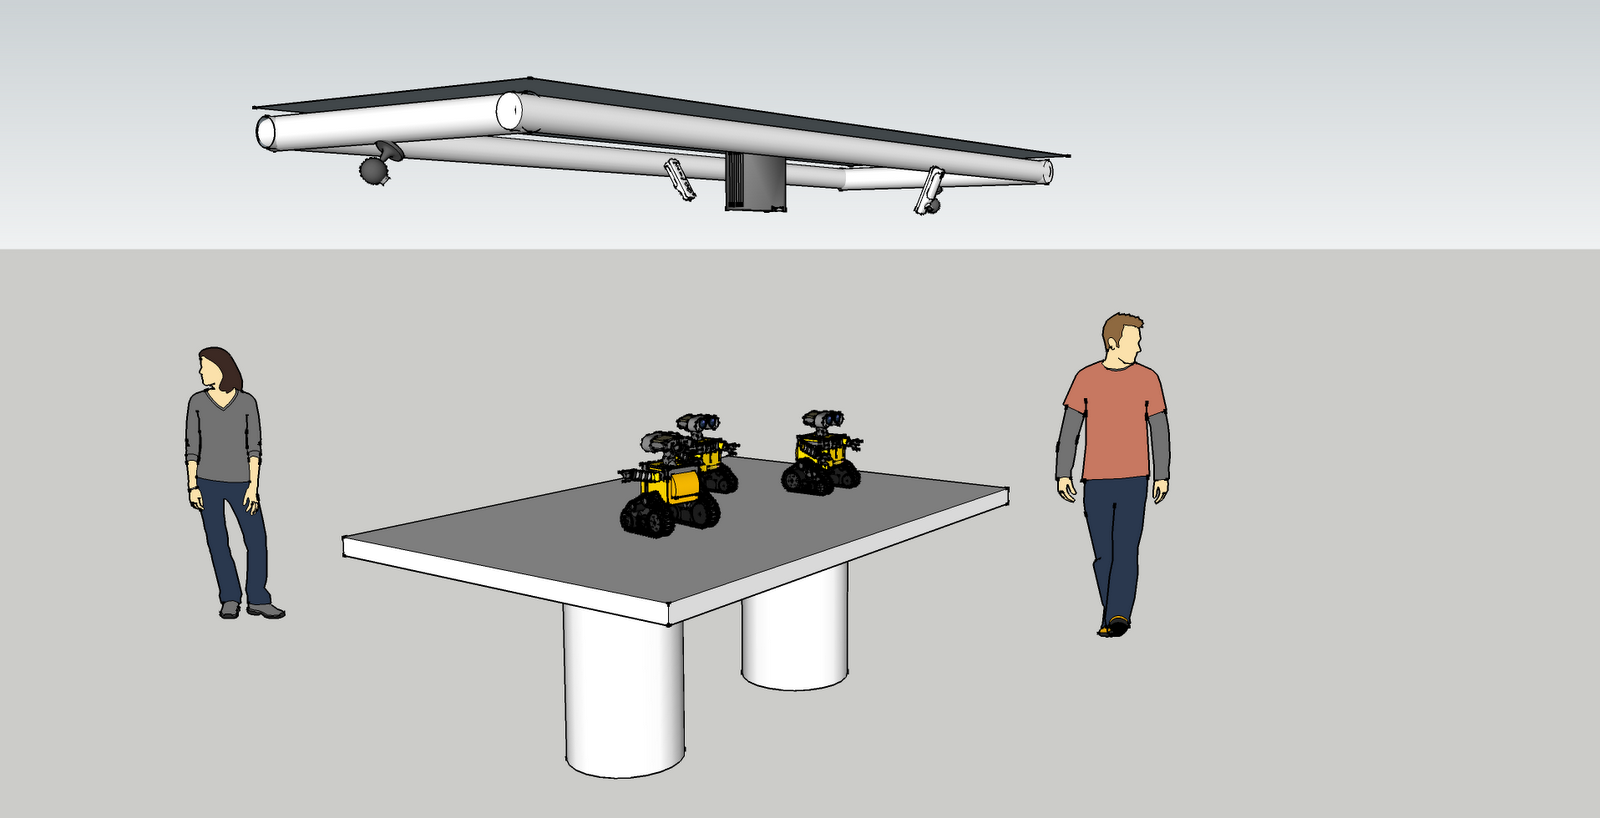
\includegraphics[width=0.8\textwidth]{./Figures/setup.png}
		\rule{35em}{0.5pt}
	\caption[Setup]{Setup a montarse para hacer estudios de grupos de robots.}
	\label{fig:setup}
\end{figure}

La función principal de MODI es ser una plataforma móvil de fácil acceso. Existe un repositorio en GitHub donde se tienen los códigos actualizados para controlar y construir robots MODI.  

\textbf{Las funciones principales que se desarrollaron}

\begin{itemize}
\item Carga Autónoma con celda solar.
\item Seguimiento de grupo.
\item Control individual del color de cada MODI.
\item Movimiento simple de cada robot de forma independiente.
\end{itemize}

%-----------------------------------
%	SECTION 2
%-----------------------------------

\section{Construcción}

%-----------------------------------
%	SUBSECTION 2
%-----------------------------------
\subsection{Fabricación Digital vs Análoga}
Cuando se quiere pasar una idea al mundo real es necesario un proceso de fabricación. Dependiendo de la cantidad de herramientas que se tenga es más o menos fácil la tarea. Desde el comienzo hasta hace un par de años, quienes se dedican a construir robots, debían construir de manera “artesanal” donde es imposible que las piezas queden todas iguales y el tiempo empleado era bastante. Hoy en día existe una gran alternativa que surge como un nuevo paradigma, la Fabricación Digital. Las llamadas impresoras 3D, que no son más que un extrusor montado en un sistema con ejes que le dan 3 grados de libertad, permiten desde un modelo hecho en un computador, obtener un modelo real en plástico. También existe otro tipo de máquinas que permite hacer diseños en 2D, estas son las cortadoras LASER. La primera versión de MODI fue construido usando planchas de madera MDF y acrílico, cortados en LASER.

\begin{figure}[htbp]
	\centering
		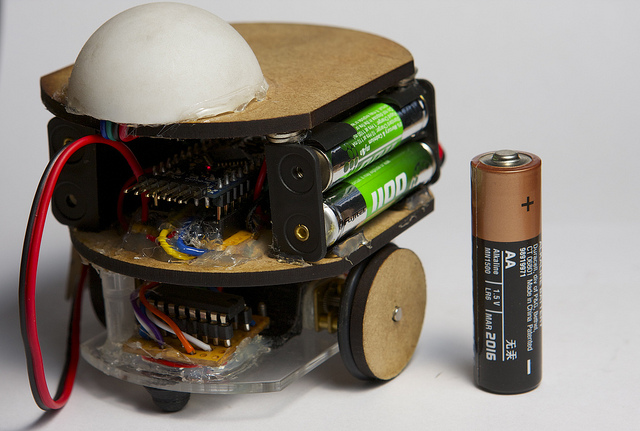
\includegraphics[width=0.8\textwidth]{./Pictures/MODIrev1.jpg}
		\rule{35em}{0.5pt}
	\caption[modi]{Primera versión robot MODI, tiene un Arduino mini pro, Xbee, usa pilas AAA y parte del chasis es de Madera MDF de 3[mm] cortado con LASER}
	\label{fig:modi}
\end{figure}

\begin{figure}[htbp]
	\centering
		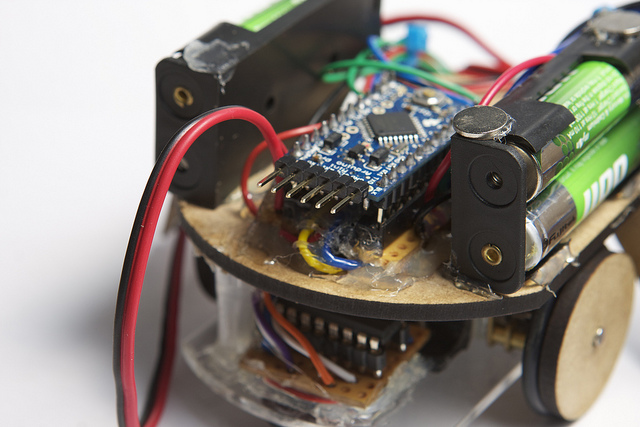
\includegraphics[width=0.8\textwidth]{./Pictures/2MODIrev1.jpg}
		\rule{35em}{0.5pt}
	\caption[modi2]{MODI, primera versión basada en gran parte en Fabricación Análoga.}
	\label{fig:modi2}
\end{figure}

\begin{figure}[htbp]
	\centering
		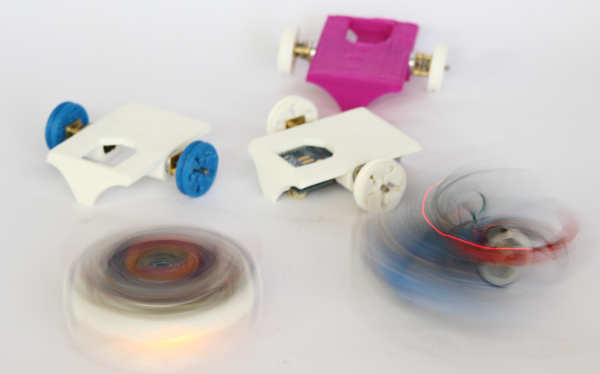
\includegraphics[width=0.8\textwidth]{./Pictures/MODIrev2.png}
		\rule{35em}{0.5pt}
	\caption[modirev1]{Primera versión de MODI usando técnica de \emph{ Fabricación Digital }con chasis de plástico construido con una MakerBot Replicator 1}
	\label{fig:modirev2}
\end{figure}

\begin{figure}[htbp]
	\centering
		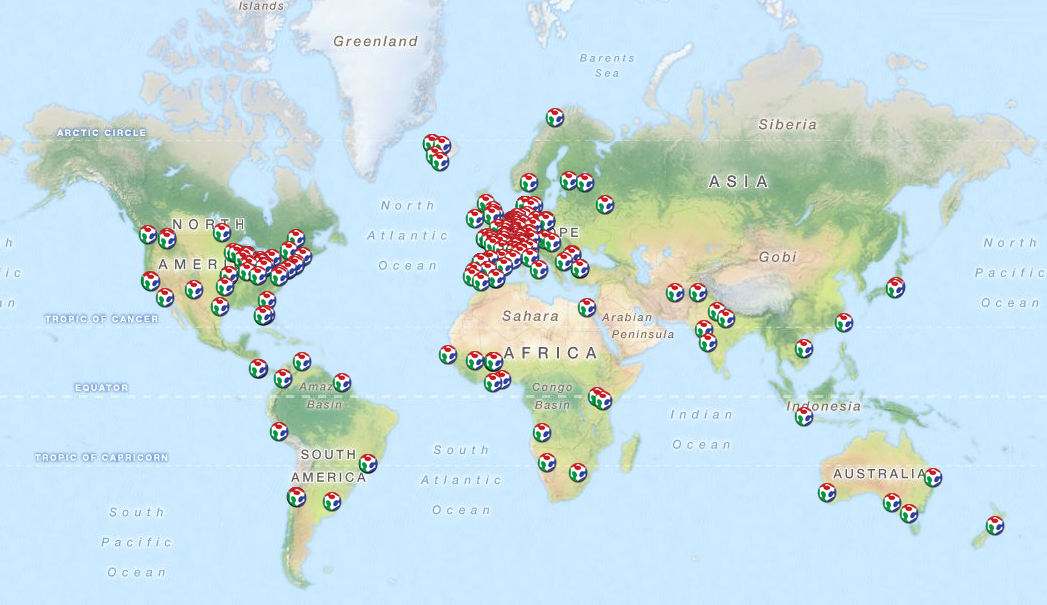
\includegraphics[width=0.8\textwidth]{./Figures/map.png}
		\rule{35em}{0.5pt}
	\caption[modirev1]{Mapa actual de lugares en el mundo que cuentan con un FabLab. En Chile a la fecha existen 3. Imagen obtenida desde http://fablabamersfoort.nl/fablabs/}
	\label{fig:Fablabs}
\end{figure}	

%-----------------------------------
%	SUBSECTION 3
%-----------------------------------
\subsection{Software CAD}

CAD hace referencia a sus siglas del inglés, Computer-aided design, y se refiere a un diseño asistido por herramientas computacionales. Profesionales como ingenieros, arquitectos y del área del diseño por lo general son los que hacen más uso de estas herramientas.

Según Wikipedia, ”... se pueden dividir básicamente en programas de dibujo en dos dimensiones (2D) y modeladores en tres dimensiones (3D). Las herramientas de dibujo en 2D se basan en entidades geométricas vectoriales como puntos,líneas, arcos y polígonos, con las que se puede operar a través de una interfaz gráfica....”

Durante el transcurso del proyecto se trabajó con 3 softwares CAD. El primero fué SketchUp 8 de Google, que permite fácilmente hacer bocetos de lugares y cuenta con una importante biblioteca de modelos para incluir en el diseño.

 ~\ref{fig:Fablabs}

